\chapter{Introduction}
\begin{refsection}
\section{Background of the Problem}

It is common knowledge that the star closest to Earth is the Sun, and also that the Sun is yellow. It is this yellow sunlight which is interesting for some of its properties \cite{onate_exploring_2021} \cite{scholes2011lessons}. For instance, plants, algae, and cyanobacteria convert this light into energy via photosynthesis. In \ref{fig:firstFig} is a photo of a galaxy which contains many stars.


\begin{equation}
	x = \frac{-b \pm \sqrt{b^2 - 4ac}}{2a}
\end{equation}


\begin{figure}[ht]
    \centering
	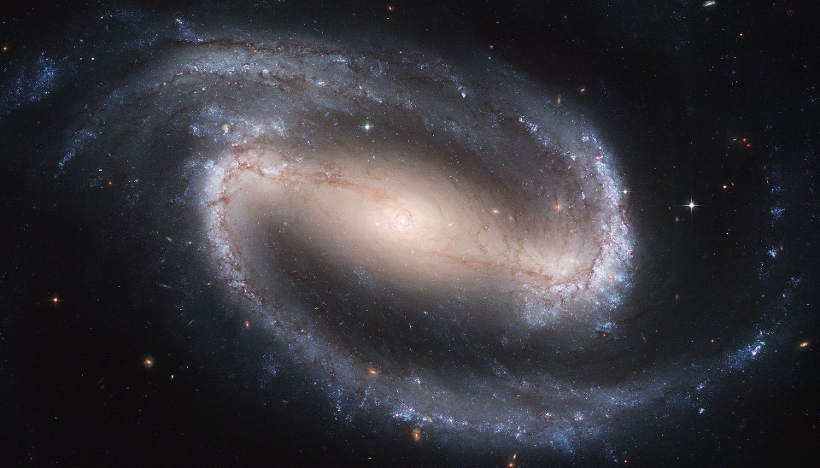
\includegraphics[width=0.85\textwidth]{figures/sampleFig1.jpg} 
	\caption[Barred spiral galaxy NGC 1300]{Barred spiral galaxy NGC 1300}
	\label{fig:firstFig}
\end{figure}

\ref{fig:firstFig}

The stars in the sky are of particular interest to the aptly named S.T.A.R. Labs, which in many recent experiments has shown promising results in converting this energy in a non-photoelectric sense into usable energy \cite{ssdsdsd_solid_2012}. Interestingly, \gls{starlabs} has theorized that the famous superhero known as ``Superman'' converts the light from our sun, which grants his fantastic abilities. There are many methods in industry for converting the sun's energy (of about \SI{1000}{\watt\per\meter\squared}) into electrical energy. Some of these are highlighted in \ref{tbl:sampleTbl1} \cite{noauthor_techopedia_nodate}.

\begin{table}[ht]
\centering
\caption{This is a table}
\label{tbl:sampleTbl1}
\resizebox{0.8\textwidth}{!}{%
\begin{tabular}{llll}
\hline
installation & type & capacity (GW) & location \\ \hline
Longyangxia Dam & photovoltaic & 0.85 & China \\
Gansu Wind Farm & wind & 6 & China \\
Sihwa Lake & tidal & 0.254 & South Korea \\ \hline
\end{tabular}%
}
\end{table}

\section{Statement of the Problem}

Enter the statement of the problem here. To cite a study add a bib entry in the references.bib, then use this code \cite{noauthor_biblatex_nodate} to cite the study.

\section{Objectives of the Study}

\subsection{General Objective}

Enter your General Objective here.

\subsection{Specific Objectives}

More Specifically, this study aims to:

\begin{enumerate}
    \item To write this research paper
    \item To present it in the title defense.
\end{enumerate}
   

\section{Significance of the Study}

Write your Significance of the study here.

\section{Scope and Limitation}

State the scope and limitation of your study here.

\section{Project Dictionary}

The Project Dictionary contains the technical terms that defined the conceptual and operation of this study:

\begin{itemize}
    \item \textbf{Convolutional Neural Network (CNN, or ConvNet).} is a class of artificial neural network, most commonly applied to analyze visual imagery. They are also known as shift invariant or space invariant artificial neural networks (SIANN), based on the shared-weight architecture of the convolution kernels or filters that slide along input features and provide translation equivariant responses known as feature maps.
    \item \textbf{Digital image processing} is the use of a digital computer to process digital images through an algorithmis the use of a digital computer to process digital images through an algorithmis the use of a digital computer to process digital images through an algorithmis the use of a digital computer to process digital imais the use of a digital computer to process digital images through an algorithmis the use of a digital computer to process digital images through an algorithmis the use of a digital computer to process digital images through an algorithmges through an is the use of a digital computer to process digital images is the use of a digital computer to process digital images through an algorithmis the use of a digital computer to process digital images through an algorithmis the use of a digital computer to process digital images through an algorithmthrough an algorithmis the use of a digital computer to process digital images through an algorithmalgorithmis the use of a digital computer to process digital images through an algorithm \cite{scholes2011lessons}. 
\end{itemize}

% Then replace \subfloat with \begin{subfigure} in your code:
	
\begin{figure}[H]
	\centering
	
	% Row 1
	\begin{subfigure}[b]{0.40\textwidth}
		\centering
		\fbox{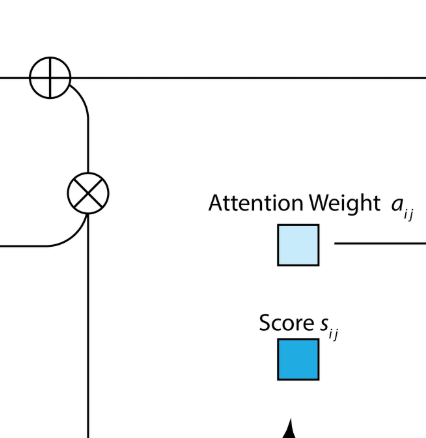
\includegraphics[width=1\textwidth]{figures/imageA.png}}
		\caption{Caption for subfigure a}
		\label{fig:firstFig:a}
	\end{subfigure}
	\hfill
	\begin{subfigure}[b]{0.40\textwidth}
		\centering
		\fbox{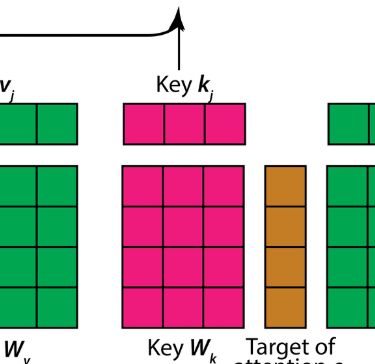
\includegraphics[width=1\textwidth]{figures/imageB.png}}
		\caption{Caption for subfigure b}
		\label{fig:firstFig:b}
	\end{subfigure}
	
	\vspace{1em}
	
	% Row 2
	\begin{subfigure}[b]{0.40\textwidth}
		\centering
		\fbox{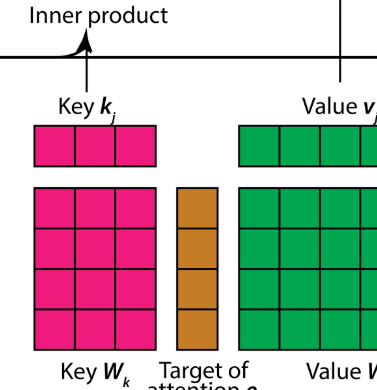
\includegraphics[width=1\textwidth]{figures/imageC.png}}
		\caption{Caption for subfigure c}
		\label{fig:firstFig:c}
	\end{subfigure}
	\hfill
	\begin{subfigure}[b]{0.40\textwidth}
		\centering
		\fbox{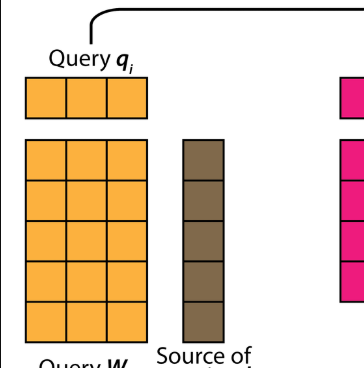
\includegraphics[width=1\textwidth]{figures/imageD.png}}
		\caption{Caption for subfigure d}
		\label{fig:firstFig:d}
	\end{subfigure}
	
	\caption{Main caption for the entire figure showcasing four different aspects.}
	\label{fig:subsubfigwithlabel}
\end{figure}


This is sample in-text citation of \ref{fig:subsubfigwithlabel} and \ref{fig:firstFig:d}.



%=======================================================%
%%%%% Do not delete this part %%%%%%
\clearpage

\printbibliography[heading=subbibintoc, title={\texorpdfstring{\centering}{} Notes}]
\end{refsection}